%%
%% Automatically generated file from DocOnce source
%% (https://github.com/hplgit/doconce/)
%%

% #define PREAMBLE

% #ifdef PREAMBLE
%-------------------- begin preamble ----------------------

\documentclass[%
oneside,                 % oneside: electronic viewing, twoside: printing
final,                   % draft: marks overfull hboxes, figures with paths
10pt]{article}

\listfiles               %  print all files needed to compile this document

\usepackage{relsize,makeidx,color,setspace,amsmath,amsfonts,amssymb}
\usepackage[table]{xcolor}
\usepackage{bm,ltablex,microtype}

\usepackage[pdftex]{graphicx}
\usepackage{fancyvrb}

\usepackage[T1]{fontenc}
%\usepackage[latin1]{inputenc}
\usepackage{ucs}
\usepackage[utf8x]{inputenc}

\usepackage{lmodern}         % Latin Modern fonts derived from Computer Modern

% Hyperlinks in PDF:
\definecolor{linkcolor}{rgb}{0,0,0.4}
\usepackage{hyperref}
\hypersetup{
    breaklinks=true,
    colorlinks=true,
    linkcolor=linkcolor,
    urlcolor=linkcolor,
    citecolor=black,
    filecolor=black,
    %filecolor=blue,
    pdfmenubar=true,
    pdftoolbar=true,
    bookmarksdepth=3   % Uncomment (and tweak) for PDF bookmarks with more levels than the TOC
    }
%\hyperbaseurl{}   % hyperlinks are relative to this root

\setcounter{tocdepth}{2}  % levels in table of contents

% Tricks for having figures close to where they are defined:
% 1. define less restrictive rules for where to put figures
\setcounter{topnumber}{2}
\setcounter{bottomnumber}{2}
\setcounter{totalnumber}{4}
\renewcommand{\topfraction}{0.95}
\renewcommand{\bottomfraction}{0.95}
\renewcommand{\textfraction}{0}
\renewcommand{\floatpagefraction}{0.75}
% floatpagefraction must always be less than topfraction!
% 2. ensure all figures are flushed before next section
\usepackage[section]{placeins}
% 3. enable begin{figure}[H] (often leads to ugly pagebreaks)
%\usepackage{float}\restylefloat{figure}

% --- fancyhdr package for fancy headers ---
\usepackage{fancyhdr}
\fancyhf{} % sets both header and footer to nothing
\renewcommand{\headrulewidth}{0pt}
\fancyfoot[LE,RO]{\thepage}
% Ensure copyright on titlepage (article style) and chapter pages (book style)
\fancypagestyle{plain}{
  \fancyhf{}
  \fancyfoot[C]{{\footnotesize \copyright\ 2018-2020, Christian Forssén. Released under CC Attribution-NonCommercial 4.0 license}}
%  \renewcommand{\footrulewidth}{0mm}
  \renewcommand{\headrulewidth}{0mm}
}
% Ensure copyright on titlepages with \thispagestyle{empty}
\fancypagestyle{empty}{
  \fancyhf{}
  \fancyfoot[C]{{\footnotesize \copyright\ 2018-2020, Christian Forssén. Released under CC Attribution-NonCommercial 4.0 license}}
  \renewcommand{\footrulewidth}{0mm}
  \renewcommand{\headrulewidth}{0mm}
}

\pagestyle{fancy}


\usepackage[framemethod=TikZ]{mdframed}

% --- begin definitions of admonition environments ---

% Admonition style "mdfbox" is an oval colored box based on mdframed
% "notice" admon
\definecolor{mdfbox_notice_background}{rgb}{1,1,1}
\newmdenv[
  skipabove=15pt,
  skipbelow=15pt,
  outerlinewidth=0,
  backgroundcolor=mdfbox_notice_background,
  linecolor=black,
  linewidth=2pt,       % frame thickness
  frametitlebackgroundcolor=mdfbox_notice_background,
  frametitlerule=true,
  frametitlefont=\normalfont\bfseries,
  shadow=false,        % frame shadow?
  shadowsize=11pt,
  leftmargin=0,
  rightmargin=0,
  roundcorner=5,
  needspace=0pt,
]{notice_mdfboxmdframed}

\newenvironment{notice_mdfboxadmon}[1][]{
\begin{notice_mdfboxmdframed}[frametitle=#1]
}
{
\end{notice_mdfboxmdframed}
}

% Admonition style "mdfbox" is an oval colored box based on mdframed
% "summary" admon
\definecolor{mdfbox_summary_background}{rgb}{1,1,1}
\newmdenv[
  skipabove=15pt,
  skipbelow=15pt,
  outerlinewidth=0,
  backgroundcolor=mdfbox_summary_background,
  linecolor=black,
  linewidth=2pt,       % frame thickness
  frametitlebackgroundcolor=mdfbox_summary_background,
  frametitlerule=true,
  frametitlefont=\normalfont\bfseries,
  shadow=false,        % frame shadow?
  shadowsize=11pt,
  leftmargin=0,
  rightmargin=0,
  roundcorner=5,
  needspace=0pt,
]{summary_mdfboxmdframed}

\newenvironment{summary_mdfboxadmon}[1][]{
\begin{summary_mdfboxmdframed}[frametitle=#1]
}
{
\end{summary_mdfboxmdframed}
}

% Admonition style "mdfbox" is an oval colored box based on mdframed
% "warning" admon
\definecolor{mdfbox_warning_background}{rgb}{1,1,1}
\newmdenv[
  skipabove=15pt,
  skipbelow=15pt,
  outerlinewidth=0,
  backgroundcolor=mdfbox_warning_background,
  linecolor=black,
  linewidth=2pt,       % frame thickness
  frametitlebackgroundcolor=mdfbox_warning_background,
  frametitlerule=true,
  frametitlefont=\normalfont\bfseries,
  shadow=false,        % frame shadow?
  shadowsize=11pt,
  leftmargin=0,
  rightmargin=0,
  roundcorner=5,
  needspace=0pt,
]{warning_mdfboxmdframed}

\newenvironment{warning_mdfboxadmon}[1][]{
\begin{warning_mdfboxmdframed}[frametitle=#1]
}
{
\end{warning_mdfboxmdframed}
}

% Admonition style "mdfbox" is an oval colored box based on mdframed
% "question" admon
\definecolor{mdfbox_question_background}{rgb}{1,1,1}
\newmdenv[
  skipabove=15pt,
  skipbelow=15pt,
  outerlinewidth=0,
  backgroundcolor=mdfbox_question_background,
  linecolor=black,
  linewidth=2pt,       % frame thickness
  frametitlebackgroundcolor=mdfbox_question_background,
  frametitlerule=true,
  frametitlefont=\normalfont\bfseries,
  shadow=false,        % frame shadow?
  shadowsize=11pt,
  leftmargin=0,
  rightmargin=0,
  roundcorner=5,
  needspace=0pt,
]{question_mdfboxmdframed}

\newenvironment{question_mdfboxadmon}[1][]{
\begin{question_mdfboxmdframed}[frametitle=#1]
}
{
\end{question_mdfboxmdframed}
}

% Admonition style "mdfbox" is an oval colored box based on mdframed
% "block" admon
\definecolor{mdfbox_block_background}{rgb}{1,1,1}
\newmdenv[
  skipabove=15pt,
  skipbelow=15pt,
  outerlinewidth=0,
  backgroundcolor=mdfbox_block_background,
  linecolor=black,
  linewidth=2pt,       % frame thickness
  frametitlebackgroundcolor=mdfbox_block_background,
  frametitlerule=true,
  frametitlefont=\normalfont\bfseries,
  shadow=false,        % frame shadow?
  shadowsize=11pt,
  leftmargin=0,
  rightmargin=0,
  roundcorner=5,
  needspace=0pt,
]{block_mdfboxmdframed}

\newenvironment{block_mdfboxadmon}[1][]{
\begin{block_mdfboxmdframed}[frametitle=#1]
}
{
\end{block_mdfboxmdframed}
}

% --- end of definitions of admonition environments ---

% prevent orhpans and widows
\clubpenalty = 10000
\widowpenalty = 10000

% --- end of standard preamble for documents ---


\usepackage[swedish]{babel}

\raggedbottom
\makeindex
\usepackage[totoc]{idxlayout}   % for index in the toc
\usepackage[nottoc]{tocbibind}  % for references/bibliography in the toc

%-------------------- end preamble ----------------------

\begin{document}

% matching end for #ifdef PREAMBLE
% #endif

\newcommand{\exercisesection}[1]{\subsection*{#1}}

\input{newcommands_keep}

% ------------------- main content ----------------------



% ----------------- title -------------------------

\thispagestyle{empty}

\begin{center}
{\LARGE\bf
\begin{spacing}{1.25}
Learning from data: Bayesian Neural Networks
\end{spacing}
}
\end{center}

% ----------------- author(s) -------------------------

\begin{center}
{\bf Christian Forssén}
\end{center}

    \begin{center}
% List of all institutions:
\centerline{{\small Department of Physics, Chalmers University of Technology, Sweden}}
\end{center}
    
% ----------------- end author(s) -------------------------

% --- begin date ---
\begin{center}
Oct 19, 2020
\end{center}
% --- end date ---

\vspace{1cm}


% !split
\section{Bayesian neural networks}
The introduction part of this lecture is inspired by the chapter \emph{"Learning as Inference"} in the excellent book \href{{http://www.inference.org.uk/mackay/itila/}}{Information Theory, Inference, and Learning Algorithms} by David MacKay.

Some python libraries that are relevant for Bayesian Neural Networks (as part of the general trend towards Probabilistic Programming in Machine Learning) are:
\begin{itemize}
\item \href{{https://docs.pymc.io/}}{PyMC3}

\item \href{{https://www.tensorflow.org/probability}}{Tensorflow Probability}

\item \href{{https://keras.io/}}{Keras} (for constructing tensorflow models).

\item \href{{http://edwardlib.org/}}{Edward}
\end{itemize}

\noindent
% !split
\subsection{Basic neural network}
We will consider a neuron with a vector of $I$ input signals $\boldsymbol{x} = \left\{ \boldsymbol{x}^{(i)} \right\}_{i=1}^I$, and an output signal $y^{(i)}$, which is given by the non-linear function $y(a)$ of the \emph{activation}
\[ a = w_0 +  \sum_{i=1}^I w_i x_i, \]
where $\boldsymbol{w} = \left\{ w_i \right\}_{i=1}^I$ are the weights of the neuron and we have included a bias ($b \equiv w_0$).

The training of the network implies feeding it with training data and finding the sets of weights and biases that minimizes a loss function that has been selected for that particular problem.
Consider, e.g., a classification problem where the single output $y$ of the final network layer is a real number $\in [0,1]$ that indicates the (discrete) probability for input $\boldsymbol{x}$ belonging to either class $t=1$ or $t=0$:
\begin{align}
p_{t=1} \equiv p(t=1 | \boldsymbol{w},\boldsymbol{x}) &= y \\
p_{t=0} \equiv p(t=0 | \boldsymbol{w},\boldsymbol{x}) &= 1-y,
\end{align}
A simple binary classifier can be trained by minimizing the loss function
\[ C_W(\boldsymbol{w}) = C(\boldsymbol{w}) +  \alpha E_W(\boldsymbol{w}), \]
made up of an error function
\[ C(\boldsymbol{w}) = -\sum_n \left[ t^{(n)} \log ( y(\boldsymbol{x}^{(n)},\boldsymbol{w})) + (1 - t^{(n)}) \log (1 - y(\boldsymbol{x}^{(n)},\boldsymbol{w})) \right], \]
where $t^{(n)}$ is the training data, and the regularizer
\[ E_W(\boldsymbol{w}) = \frac{1}{2} \sum_i w_i^2, \]
that is designed to avoid overfitting.
The error function can be interpreted as minus the log likelihood
\[ p(\mathcal{D}|\boldsymbol{w}) = \exp\left[ - C(\boldsymbol{w}) \right]. \]
Similarly the regularizer can be interpreted in terms of a log prior probability distribution over the parameters
\[ p(\boldsymbol{w} | \alpha) = \frac{1}{Z_W(\alpha)} \exp \left[ -\alpha E_W \right]. \]
If $E_W$ is quadratic as given above, then the corresponding prior distribution is a Gaussian with variance $\sigma_W^2 = 1/\alpha$ and $1/Z_W = (\alpha/2\pi)^{K/2}$, where $K$ is the number of parameters in $w$.
The objective function $C_W(w)$ then corresponds to the inference of the parameters $\boldsymbol{w}$ given the data
\[ p(\boldsymbol{w} | \mathcal{D}, \alpha) = \frac{p(D|\boldsymbol{w}) p(\boldsymbol{w}|\alpha)}{p(\mathcal{D}|\alpha)} = \frac{1}{Z_M} \exp [ -C_W(\boldsymbol{w}) ]. \]
We show the evolution of the probability distribution for a sequence of an increasing number of training data in the following figure. The network parameters $\boldsymbol{w}$ that are found by minimizing $C_W(\boldsymbol{w})$ can be interpreted as the (locally) most probable parameter vector $\boldsymbol{w}^*$.


\begin{figure}[!ht]  % 
  \centerline{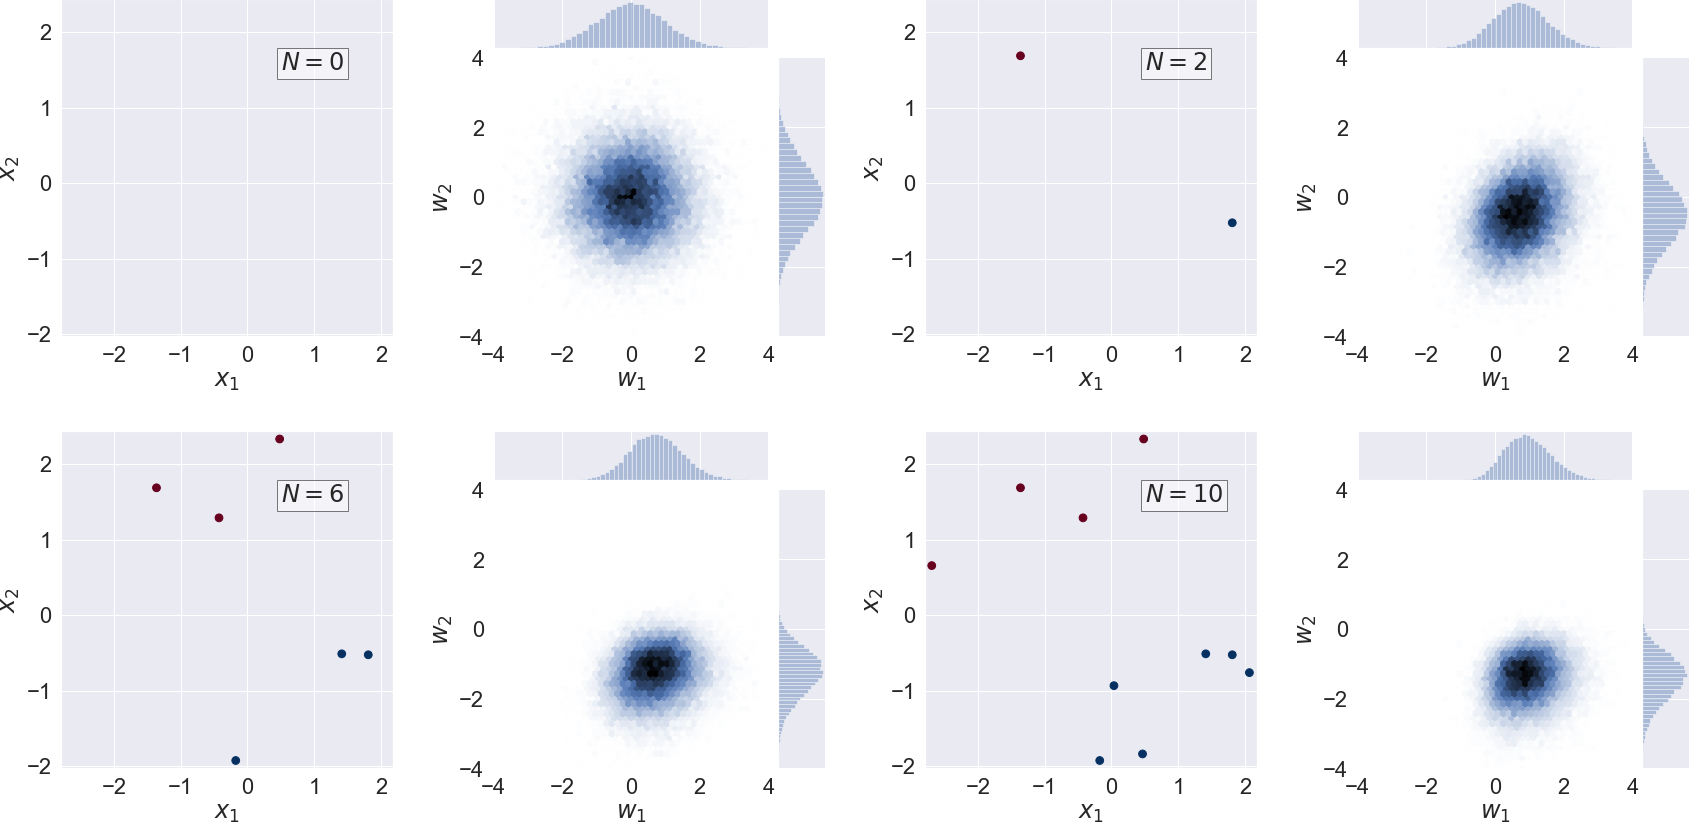
\includegraphics[width=0.95\linewidth]{fig/scatter_joint_bnn_plot.png}}
  \caption{
  Scatter plot of training data and the corresponding bivariate posterior pdf for the neuron weights $p(w_1, w_2 | \mathcal{D}, \alpha)$ (i.e.~marginalized over the bias $w_0$) for a sequence of $N=0,2,6,10$ training data.
  }
\end{figure}
%\clearpage % flush figures 


Instead, we will use the Bayesian approach and consider the information that is contained in the actual probability distribution. In fact, there are different uncertainties that should be addressed:

\begin{description}
\item[Epistemic uncertainties:] 
  from uncertainties in the model. For a neural network, this uncertainty can, in principle, be reduced with more data and quantified using the Bayesian approach. Epistemic uncertainty is also known as \textbf{systematic uncertainty}.

\item[Aleatoric uncertainties:] 
  from inherent noise in the training data. This should be included in the likelihood function (and is therefore part of the Bayesian approach). It can, however, not be reduced with more data of the same quality. Aleatoric uncertainty is also known as \textbf{statistical uncertainty}. Aleatoric is derived from the Latin \emph{alea} or dice, referring to a game of chance.
\end{description}

\noindent

\begin{notice_mdfboxadmon}[Notice]
We will use $y$ to denote the output from the neural network. For classification problems, $y$ will give the categorical (discrete) distribution of probabilities $p_{t=c}$ of belonging to class $c$. For regression problems, $y$ is a continuous variable. It could also, in general, be a vector of outputs. The neural network can be seen as a non-linear mapping $y(x; w)$: $x \in \mathbb{R}^p \to y \in \mathbb{R}^m$.
\end{notice_mdfboxadmon} % title: Notice



% !split
\subsection{Probabilistic model}

A Bayesian neural network can be viewed as probabilistic model in which we want to infer $p(y \lvert \boldsymbol{x},\mathcal{D})$ where $\mathcal{D} = \left\{\boldsymbol{x}^{(i)}, y^{(i)}\right\}$ is a given training dataset. 

We construct the likelihood function $p(\mathcal{D} \lvert \boldsymbol{w}) = \prod_i p(y^{(i)} \lvert \boldsymbol{x}^{(i)}, \boldsymbol{w})$ which is a function of parameters $\boldsymbol{w}$. Maximizing the likelihood function gives the maximimum likelihood estimate (MLE) of $\boldsymbol{w}$. The usual optimization objective during training is the negative log likelihood. For a categorical distribution this is the \emph{cross entropy} error function, for a Gaussian distribution this is proportional to the \emph{sum of squares} error function. MLE can lead to severe overfitting though.

Multiplying the likelihood with a prior distribution $p(\boldsymbol{w})$ is, by Bayes theorem, proportional to the posterior distribution $p(\boldsymbol{w} \lvert \mathcal{D}) \propto p(\mathcal{D} \lvert \boldsymbol{w}) p(\boldsymbol{w})$. Maximizing $p(\mathcal{D} \lvert \boldsymbol{w}) p(\boldsymbol{w})$ gives the maximum a posteriori (MAP) estimate of $\boldsymbol{w}$. Computing the MAP estimate has a regularizing effect and can prevent overfitting. The optimization objectives here are the same as for MLE plus a regularization term coming from the log prior.

Both MLE and MAP give point estimates of parameters. If we instead had a full posterior distribution over parameters we could make predictions that take weight uncertainty into account. This is covered by the posterior predictive distribution $p(y \lvert \boldsymbol{x},\mathcal{D}) = \int p(y \lvert \boldsymbol{x}, \boldsymbol{w}) p(\boldsymbol{w} \lvert \mathcal{D}) d\boldsymbol{w}$ in which the parameters have been marginalized out. This is equivalent to averaging predictions from an ensemble of neural networks weighted by the posterior probabilities of their parameters $\boldsymbol{w}$.

Returning to the binary classification problem, $y^{(n+1)}$ corresponds to the probability $p_{t^{(n+1)}=1}$ and a Bayesian prediction of a new datum $y^{(n+1)}$ will correspond to a pdf and involves \emph{marginalizing} over the weight and bias parameters
\[ p(y^{(n+1)} | x^{(n+1)}, D, \alpha) = \int d \boldsymbol{w} p( y^{(n+1)} | x^{(n+1)}, w, \alpha) p(w|D,\alpha), \]
where we have also included the weight decay hyperparameter $\alpha$ from the prior (regularizer). Marginalization could, of course, also be performed over this parameter.

We show an example of such inference, comparing the point estimate $y(x; w^*, \alpha)$ and the Bayesian approach, in the following figure.


\begin{figure}[!ht]  % 
  \centerline{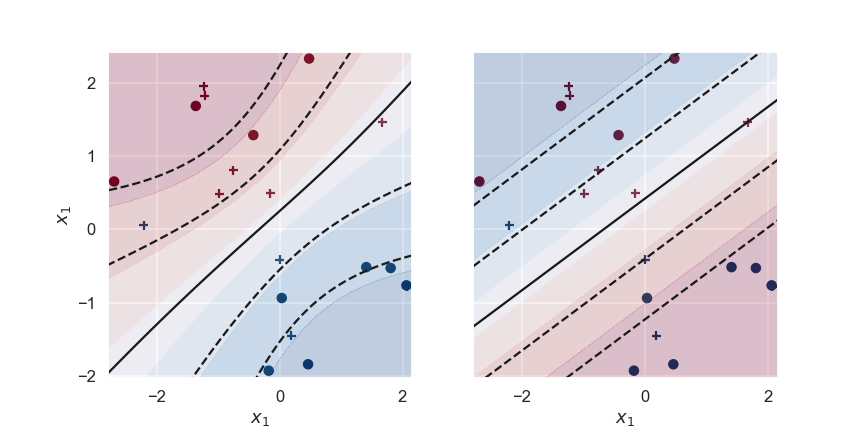
\includegraphics[width=0.95\linewidth]{fig/bnn_binary_classifier_mean.png}}
  \caption{
  The predictions for a Bayesian (left panel) and regular (right panel) binary classifier that has been learning from ten training data (circles) with a weight decay $\alpha = 1.0$. The decision boundary ($y=0.5$, i.e.~the activation $a=0$) is shown together with the levels 0.12,0.27,0.73,0.88 (corresponding to the activation $a=\pm1,\pm2$). Test data is shown as plus symbols.
  }
\end{figure}
%\clearpage % flush figures 


The Bayesian classifier is based on sampling a very large ensamble of single neurons with different parameters. The distribution of these samples will be proportional to the posterior pdf for the parameters. The decision boundary shown in the figure is obtained as the mean of the predictions of the sampled neurons evaluated on a grid. It is clear that the Bayesian classifier is more uncertain about its predictions in the lower left and upper right corners, where there is little training data. 

This becomes even more clear when we plot the standard deviation of the predictions of the Bayesian classifier.


\begin{figure}[!ht]  % 
  \centerline{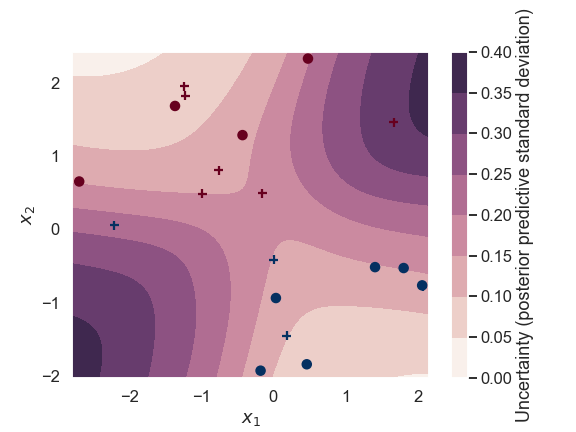
\includegraphics[width=0.8\linewidth]{fig/bnn_binary_classifier_stddev.png}}
  \caption{
  The standard deviation of the class label predictions for a Bayesian binary classifier.
  }
\end{figure}
%\clearpage % flush figures 


The predictions are rather certain along a diagonal line (close to the training data). Note that the interpretation of the prediction in the center of the figure (near $x_1,x_2 = 0,0$) is the following: The Bayesian binary classifier predicts a probability of $\sim 0.5$ for this point in the input parameter space to belong to class 1 (i.e.~the decision is very uncertain). The Baysian classifier is also very certain about this uncertainty (the standard deviation is small).

In contrast, predictions for points in the upper left or lower right corners are very certain about the class label (and there is little uncertainty about this certainty).



% !split
\subsection{Bayesian neural networks in practice}
But how shall we compute the marginalization integral for serious neural networks with thousands of parameters?

In short, there are three different approaches:

\begin{enumerate}
\item \textbf{Sampling methods}, e.g.~MCMC sampling (this approach would be exact as the number of samples $\rightarrow \infty$);

\item \textbf{Deterministic approximate methods}, for example using Gaussian approximations with the Laplace method;

\item \textbf{Variational methods}.
\end{enumerate}

\noindent
The first two are discussed in MacKay's book, while we will focus on the variational methods in the following.

% !split
\subsection{Variational inference for Bayesian neural networks}

Bayesian neural networks differ from plain neural networks in that their weights are assigned a probability distribution instead of a single value or point estimate. These probability distributions describe the uncertainty in weights and can be used to estimate uncertainty in predictions. Training a Bayesian neural network via variational inference learns the parameters of these distributions instead of the weights directly.

Unfortunately, an analytical solution for the weight posterior $p(\boldsymbol{w} \lvert \mathcal{D})$ in neural networks is intractable. We therefore have to approximate the true posterior with a proxy variational distribution $q(\boldsymbol{w} \lvert \boldsymbol{\theta})$ whose parameters we want to estimate. 

This can be done by minimizing the \href{{https://en.wikipedia.org/wiki/Kullback%E2%80%93Leibler_divergence}}{Kullback-Leibler divergence} between $q(\boldsymbol{w} \lvert \boldsymbol{\theta})$ and the true posterior $p(\boldsymbol{w} \lvert \mathcal{D})$  w.r.t. $\boldsymbol{\theta}$.

The specific goal is then to replace $p(\boldsymbol{w} \lvert \mathcal{D})$, which we don't know, with the known proxy distribution $q(\boldsymbol{w} \lvert \boldsymbol{\theta}^*)$, where $\boldsymbol{\theta}^*$ is the optimal set of variational parameters. 

% !split
\paragraph{The Kullback-Leibler divergence.}
The KL divergence is a numeric measure of the difference between two distributions. For two probability distributions $q(\boldsymbol{w})$ and $p(\boldsymbol{w})$, the KL divergence in a continuous case,
\[ D_\mathrm{KL}(q||p) = \int d \boldsymbol{w} q(\boldsymbol{w}) \log \frac{q(\boldsymbol{w})}{p(\boldsymbol{w})} \equiv \mathbb{E}_{q} \left[ \log \, q(\boldsymbol{w}) - \log \, p(\boldsymbol{w}) \right] \]
As we can see, the KL divergence calculates the expected log differences in between two distributions with respect to distribution q. It is a non-negative quantity and it is equal to zero only when the two distributions are identical.

Intuitively there are three scenarios:
\begin{itemize}
\item if both $q$ and $p$ are high at the same positions, then we are happy;

\item if $q$ is high where $p$ is low, we pay a price;

\item if $q$ is low we don't care (because of the expectation).
\end{itemize}

\noindent
The divergence measure is not symmetric, i.e., $D_\mathrm{KL}(p||q) \neq D_\mathrm{KL}(q||p)$. In fact, it is possibly more natural to reverse the arguments and compute $D_\mathrm{KL}(p||q)$. However, we choose $\mathrm{KL}(q||p)$ so that we can take expectations with respect to the known $q(\boldsymbol{w})$ distribution. In addition, the minimization of this KL divergence will encourage the fit to concentrate on plausible parameters since
\[
D_\mathrm{KL}(q||p) = \int d \boldsymbol{w} q(\boldsymbol{w}\lvert \boldsymbol{\theta}) \log \frac{q(\boldsymbol{w} \lvert \boldsymbol{\theta})}{p(\boldsymbol{w} \lvert \mathcal{D})} 
= -\int d \boldsymbol{w} q(\boldsymbol{w}\lvert \boldsymbol{\theta}) \log \, p(\boldsymbol{w} \lvert \mathcal{D}) + \int d \boldsymbol{w} q(\boldsymbol{w}\lvert \boldsymbol{\theta}) \log \, q(\boldsymbol{w} \lvert \boldsymbol{\theta}).
\]
To minimize the first term we have to avoid putting probability mass into regions of implausible parameters. To minimize the second term we have to maximize the entropy of the variational distribution $q$ as this term corresponds to its negative entropy.

% !split
\paragraph{Evidence Lower Bound.}
Let us rewrite the posterior pdf $p(\boldsymbol{w} \lvert \mathcal{D})$ using Bayes theorem
\begin{align*}
D_\mathrm{KL}(q||p) &= \int d \boldsymbol{w} q(\boldsymbol{w}\lvert \boldsymbol{\theta}) \left[ \log \, q(\boldsymbol{w}\lvert \boldsymbol{\theta})  - p( \mathcal{D} \lvert \boldsymbol{w}) - p(\boldsymbol{w}) + p(\mathcal{D}) \right] \\
&= \mathbb{E}_{q} \left[ \log \, q(\boldsymbol{w} \lvert \boldsymbol{\theta}) \right]
- \mathbb{E}_{q} \left[ \log \, p(\mathcal{D} \lvert \boldsymbol{w}) \right]
- \mathbb{E}_{q} \left[ \log \, p(\boldsymbol{w}) \right]
+ \log \, p(\mathcal{D}).
\end{align*}
Note that the logarithm of the last term has no dependence on $\boldsymbol{w}$ and the integration of $q$ will just give one since it should be a properly normalized pdf. This term is then the log marginal likelihood (or model evidence). Furthermore, since the KL divergence on the left hand side is bounded from below by zero we get the \textbf{Evidence Lower Bound} (ELBO)
\begin{equation}
\log \, p(\mathcal{D}) \ge 
- \mathbb{E}_{q} \left[ \log \, q(\boldsymbol{w} \lvert \boldsymbol{\theta}) \right]
+ \mathbb{E}_{q} \left[ \log \, p(\mathcal{D} \lvert \boldsymbol{w}) \right]
+ \mathbb{E}_{q} \left[ \log \, p(\boldsymbol{w}) \right]
\equiv J_\mathrm{ELBO}(\boldsymbol{\theta})
\label{eq:elbo}
\end{equation}
Variational inference was originally inspired by work in statistical physics, and with that analogy, $-J_\mathrm{ELBO}(\boldsymbol{\theta})$ is also called the \textbf{variational free energy} and sometimes denoted $\mathcal{F}(\mathcal{D},\boldsymbol{\theta})$.

The task at hand is therefore to find the set of parameters $\boldsymbol{\theta}^*$ that maximizes $J_\mathrm{ELBO}(\boldsymbol{\theta})$. The hardest term to evaluate is obviously the expectation of the log-likelihood
\[
\mathbb{E}_{q} \left[ \log \, p(\mathcal{D} \lvert \boldsymbol{w}) \right]
= \sum{i=1}^N \mathbb{E}_{q} \left[ \log \, p( y^{(i)} \lvert \boldsymbol{x}^{(i)}, \boldsymbol{w}) \right].
\]
This problem constitutes a new and active area of research in machine learning and it permeates well with the overarching theme of this course which is inference from data. We will end by giving two pointers to further readings on this subject.

% !split
\subsection{Bayesian neural networks in PyMC3}
In the demonstration notebook of this lecture, it is shown how to use Variational Inference in PyMC3 to fit a simple Bayesian Neural Network. That implementation is based on the \textbf{Automatic Differentation Variational Inference} (ADVI) approach, described e.g.~in \href{{https://arxiv.org/abs/1506.03431}}{Automatic Variational Inference in Stan}.


\begin{figure}[!ht]  % 
  \centerline{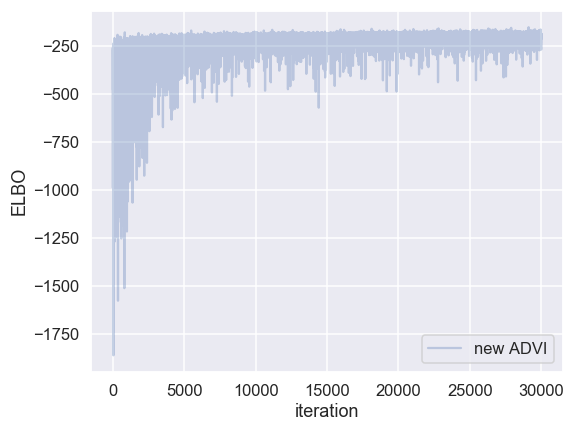
\includegraphics[width=0.6\linewidth]{fig/ADVI-classifier_ELBO.png}}
  \caption{
  The training of the Bayesian binary classifier, that employs ADVI implemented in \texttt{pymc3}, corresponds to modifying the variational distribution's hyperparameters in order to maximize the Evidence Lower Bound (ELBO).
  }
\end{figure}
%\clearpage % flush figures 



\begin{figure}[!ht]  % 
  \centerline{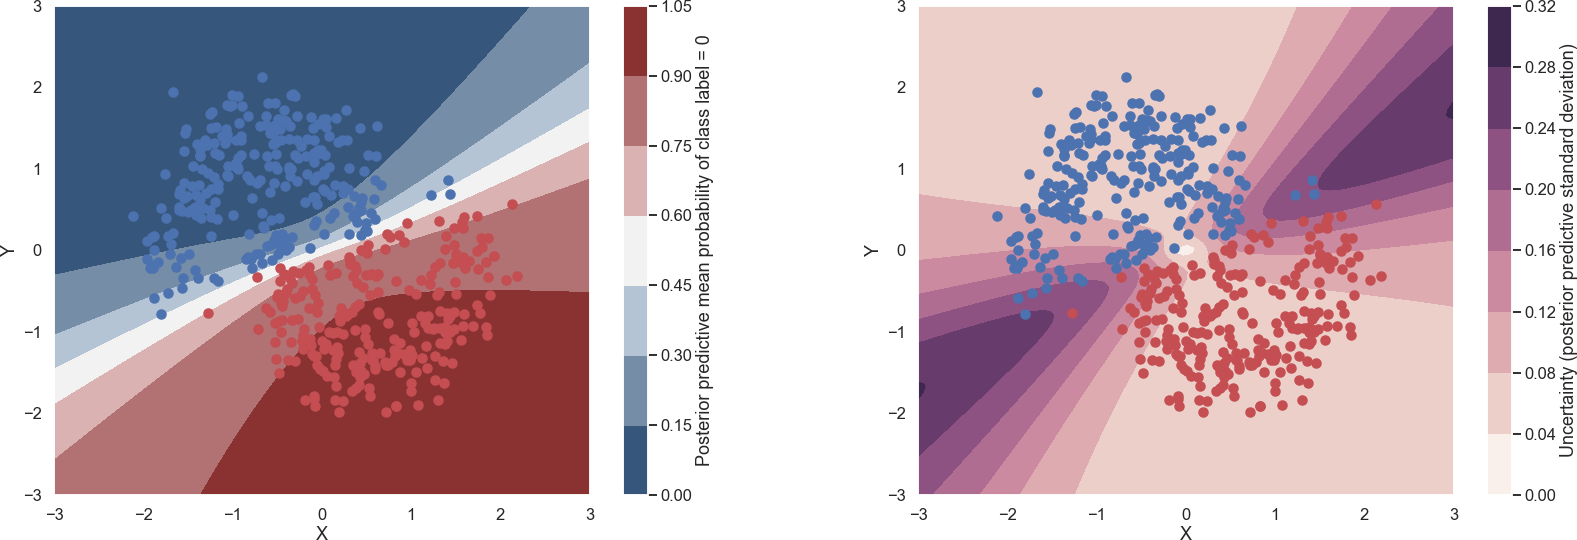
\includegraphics[width=0.95\linewidth]{fig/ADVI-classifier.png}}
  \caption{
  The predictions for a Bayesian binary classifier that has been learning using ADVI implemented in \texttt{pymc3}. The mean (left panel) and standard deviation (right panel) of the binary classifier's label predictions are shown.
  }
\end{figure}
%\clearpage % flush figures 


See also 
\begin{itemize}
\item Kucukelbir, A., Tran, D., Ranganath, R., Gelman, A., and Blei, D. M. (2016). \emph{Automatic Differentiation Variational Inference}. arXiv preprint arXiv:"1603.00788": 'https://arxiv.org/abs/1603.00788".
\end{itemize}

\noindent
% !split
\subsection{Bayes by Backprop}

The well-cited paper paper: \href{{https://arxiv.org/abs/1505.05424}}{Weight Uncertainty in Neural Networks} (\emph{Bayes by Backprop}) has been well described in the \href{{http://krasserm.github.io/2019/03/14/bayesian-neural-networks/}}{blog entry} by Martin Krasser. The main points of this blog entry are reproduced below with some modifications and some adjustments of notation. 

All three terms in equation (\ref{eq:elbo}) are expectations w.r.t. the variational distribution $q(\boldsymbol{w} \lvert \boldsymbol{\theta})$. In this paper they use the variational free energy $\mathcal{F}(\mathcal{D},\boldsymbol{\theta}) \equiv -J_\mathrm{ELBO}(\boldsymbol{\theta})$ as a cost function (since it should be \emph{minimized}). This quantity can be approximated by drawing \href{{https://en.wikipedia.org/wiki/Monte_Carlo_method}}{Monte Carlo} samples $\boldsymbol{w}^{(i)}$ from $q(\boldsymbol{w} \lvert \boldsymbol{\theta})$.

\begin{equation} 
\mathcal{F}(\mathcal{D},\boldsymbol{\theta}) \approx {1 \over N} \sum_{i=1}^N \left[
\log \, q(\boldsymbol{w}^{(i)} \lvert \boldsymbol{\theta}) -
\log \, p(\boldsymbol{w}^{(i)}) -
\log \, p(\mathcal{D} \lvert \boldsymbol{w}^{(i)})\right]
\label{eq:VariationalFreeEnergy}
\end{equation}

In the example used in the blog post, they use a Gaussian distribution for the variational posterior, parameterized by $\boldsymbol{\theta} = (\boldsymbol{\mu}, \boldsymbol{\sigma})$ where $\boldsymbol{\mu}$ is the mean vector of the distribution and $\boldsymbol{\sigma}$ the standard deviation vector. The elements of $\boldsymbol{\sigma}$ are the elements of a diagonal covariance matrix which means that weights are assumed to be uncorrelated. Instead of parameterizing the neural network with weights $\boldsymbol{w}$ directly, it is parameterized with $\boldsymbol{\mu}$ and $\boldsymbol{\sigma}$ and therefore the number of parameters are doubled compared to a plain neural network.

% !split
\paragraph{Network training.}
A training iteration consists of a forward-pass and and backward-pass. During a forward pass a single sample is drawn from the variational posterior distribution. It is used to evaluate the approximate cost function defined by equation (\ref{eq:VariationalFreeEnergy}). The first two terms of the cost function are data-independent and can be evaluated layer-wise, the last term is data-dependent and is evaluated at the end of the forward-pass. During a backward-pass, gradients of $\boldsymbol{\mu}$ and $\boldsymbol{\sigma}$ are calculated via backpropagation so that their values can be updated by an optimizer.

Since a forward pass involves a stochastic sampling step we have to apply the so-called \emph{re-parameterization trick} for backpropagation to work. The trick is to sample from a parameter-free distribution and then transform the sampled $\boldsymbol{\epsilon}$ with a deterministic function $t(\boldsymbol{\mu}, \boldsymbol{\sigma}, \boldsymbol{\epsilon})$ for which a gradient can be defined. In the blog post they choose $\boldsymbol{\epsilon}$ to be drawn from a standard normal distribution i.e.~$\boldsymbol{\epsilon} \sim \mathcal{N}(\boldsymbol{0}, \boldsymbol{I})$ and the function $t$ is taken to be $t(\boldsymbol{\mu}, \boldsymbol{\sigma}, \boldsymbol{\epsilon}) = \boldsymbol{\mu} + \boldsymbol{\sigma} \odot \boldsymbol{\epsilon}$, i.e., it shifts the sample by mean $\boldsymbol{\mu}$ and scales it with $\boldsymbol{\sigma}$ where $\odot$ is element-wise multiplication.

For numerical stability the network is parametrized with $\boldsymbol{\rho}$ instead of $\boldsymbol{\sigma}$ and $\boldsymbol{\rho}$ is transformed with the softplus function to obtain $\boldsymbol{\sigma} = \log(1 + \exp(\boldsymbol{\rho}))$. This ensures that $\boldsymbol{\sigma}$ is always positive. As prior, a scale mixture of two Gaussians is used $p(\boldsymbol{w}) = \pi \mathcal{N}(\boldsymbol{w} \lvert 0,\sigma_1^2) + (1 - \pi) \mathcal{N}(\boldsymbol{w} \lvert 0,\sigma_2^2)$ where $\sigma_1$, $\sigma_2$ and $\pi$ are shared parameters. Their values are learned during training (which is in contrast to the paper where a fixed prior is used).

See Martin Krasser's \href{{http://krasserm.github.io/2019/03/14/bayesian-neural-networks/}}{blog entry} for results and further details.

% ------------------- end of main content ---------------

% #ifdef PREAMBLE
\end{document}
% #endif

